\documentclass[
	% -- opções da classe memoir --
	12pt,				% tamanho da fonte
	%openright,			% capítulos começam em pág ímpar (insere página vazia caso preciso)
	oneside,			% para impressão em recto e verso. Oposto a oneside
	a4paper,			% tamanho do papel. 
	% -- opções da classe abntex2 --
	%chapter=TITLE,		% títulos de capítulos convertidos em letras maiúsculas
	%section=TITLE,		% títulos de seções convertidos em letras maiúsculas
	%subsection=TITLE,	% títulos de subseções convertidos em letras maiúsculas
	%subsubsection=TITLE,% títulos de subsubseções convertidos em letras maiúsculas
	% -- opções do pacote babel --
	english,			% idioma adicional para hifenização
	french,				% idioma adicional para hifenização
	spanish,			% idioma adicional para hifenização
	brazil,				% o último idioma é o principal do documento
	]{abntex2}


% ---
% PACOTES
% ---

% ---
% Pacotes fundamentais 
% ---
\usepackage{pslatex}			% Usa a fonte Latin Modern
\usepackage[T1]{fontenc}		% Selecao de codigos de fonte.
\usepackage[utf8]{inputenc}		% Codificacao do documento (conversão automática dos acentos)
\usepackage{indentfirst}		% Indenta o primeiro parágrafo de cada seção.
\usepackage{color}				% Controle das cores
\usepackage{graphicx}			% Inclusão de gráficos
\usepackage{subfig}
\usepackage{microtype} 			% para melhorias de justificação
\usepackage{transparent}
\usepackage{eso-pic}
\usepackage{amsthm,amsfonts}
\usepackage{float}

% ---

% ---
% Pacotes adicionais, usados no anexo do modelo de folha de identificação
% ---
\usepackage{multicol}
\usepackage{multirow}
% ---
	
% ---
% Pacotes adicionais, usados apenas no âmbito do Modelo Canônico do abnteX2
% ---
%\usepackage{lipsum}				% para geração de dummy text
% ---

% ---
% Pacotes de citações
% ---
\usepackage[brazilian,hyperpageref]{backref}	 % Paginas com as citações na bibl
\usepackage[alf]{abntex2cite}	% Citações padrão ABNT

% --- 
% CONFIGURAÇÕES DE PACOTES
% --- 

% ---
% Configurações do pacote backref
% Usado sem a opção hyperpageref de backref
\renewcommand{\backrefpagesname}{Citado na(s) página(s):~}
% Texto padrão antes do número das páginas
\renewcommand{\backref}{}
% Define os textos da citação
\renewcommand*{\backrefalt}[4]{
	\ifcase #1 %
		Nenhuma citação no texto.%
	\or
		Citado na página #2.%
	\else
		Citado #1 vezes nas páginas #2.%
	\fi}%
% ---

% ---
% Informações de dados para CAPA e FOLHA DE ROSTO
% ---
\titulo{Relatório sobre Cronoanálise\\Introdução a Engenharia de Produção}
\autor{Anderson Gomes da Silva RA 110826\\Eduardo Oliveira RA 108164\\Gabriel Rodrigues Munhoz RA 106802\\Guilherme Benetti RA 107613\\Hugo Minella RA 110862\\José Henrique Gonçalves RA 110058}
\local{Maringá, São Paulo}
\data{Maio de 2018}
\instituicao{%
  Universidade Estadual de Maringá - UEM
  \par
  Departamento de Engenharia de Produção - DEP}
\tipotrabalho{Relatório técnico}
% O preambulo deve conter o tipo do trabalho, o objetivo, 
% o nome da instituição e a área de concentração 
\preambulo{Aplicação da Cronoanálise em medições feitas em sala de aula para comparação da produtividade com 1, 2 e 3 funcionários}
% ---

% ---
% Configurações de aparência do PDF final

% alterando o aspecto da cor azul
\definecolor{blue}{RGB}{41,5,195}

% informações do PDF
\makeatletter
\hypersetup{
     	%pagebackref=true,
		pdftitle={\@title}, 
		pdfauthor={\@author},
    	pdfsubject={\imprimirpreambulo},
	    pdfcreator={LaTeX with abnTeX2},
		pdfkeywords={abnt}{latex}{abntex}{abntex2}{relatório técnico}, 
		colorlinks=true,       		% false: boxed links; true: colored links
    	linkcolor=blue,          	% color of internal links
    	citecolor=blue,        		% color of links to bibliography
    	filecolor=magenta,      		% color of file links
		urlcolor=blue,
		bookmarksdepth=4
}
\makeatother
% --- 

% --- 
% Espaçamentos entre linhas e parágrafos 
% --- 

% O tamanho do parágrafo é dado por:
\setlength{\parindent}{1.3cm}

% Controle do espaçamento entre um parágrafo e outro:
\setlength{\parskip}{0.2cm}  % tente também \onelineskip

% ---
% compila o indice
% ---
%\makeindex
% ---
\usepackage{fancyhdr}
\fancyhead{}
\fancyfoot{}
\lhead{Relatório sobre Cronoanálise}
\rhead{\thepage}

\AddToShipoutPicture{

\put(0,0){

\parbox[b][\paperheight]{\paperwidth}{%

\vfill

\centering

{\transparent{0.1}\includegraphics[scale=1.4]{../Imagens/marcadaguauem.jpg}   }%

\vfill}}}
% ----
% Início do documento
% ----
\graphicspath{{../Imagens}}
\begin{document}

\begin{minipage}[c][3.5cm][c]{3cm} % a primeira minipágina tem uma altura de 1.5cm e uma largura de 3cm.

\centering

\includegraphics[scale=0.4]{../Imagens/bla.png} 

\end{minipage}

% Seleciona o idioma do documento (conforme pacotes do babel)
%\selectlanguage{english}
\selectlanguage{brazil}

% Retira espaço extra obsoleto entre as frases.
\frenchspacing 

% ----------------------------------------------------------
% ELEMENTOS PRÉ-TEXTUAIS
% ----------------------------------------------------------
% \pretextual

% ---
% Capa
% ---
\imprimircapa
% ---

% ---
% Folha de rosto
% (o * indica que haverá a ficha bibliográfica)
% ---
%\imprimirfolhaderosto*

% ---
% inserir o sumario
% ---
\pdfbookmark[0]{\contentsname}{toc}
\tableofcontents*
\newpage

%\section[Objetivo]{Objetivo}
%\pagestyle{fancy}

%\newpage
\section[Introdução]{Introdução}
\pagestyle{fancy}

Bla bla


% ---
% inserir lista de ilustrações
% ---
%\pdfbookmark[0]{\listfigurename}{lof}
%\listoffigures*
%\cleardoublepage
% ---
% ---
% inserir lista de tabelas
% ---
%\pdfbookmark[0]{\listtablename}{lot}
%\listoftables*
%\cleardoublepage
% ---

% ---
% inserir lista de abreviaturas e siglas
% ---
%\begin{siglas}
% \item[ABNT] Associação Brasileira de Normas Técnicas
%  \item[abnTeX] ABsurdas Normas para TeX
%\end{siglas}
% ---

% ---
% inserir lista de símbolos
% ---
%\begin{simbolos}
  %\item[$ \Gamma $] Letra grega Gama
  %\item[$ \Lambda $] Lambda
  %\item[$ \zeta $] Letra grega minúscula zeta
  %\item[$ \in $] Pertence
%\end{simbolos}
% ---

% ----------------------------------------------------------
% ELEMENTOS TEXTUAIS
% ----------------------------------------------------------

%\newpage
%\section[Introdução Teórica]{Introdução Teórica}
%\pagestyle{fancy}


% ----------------------------------------------------------
% PARTE - preparação da pesquisa
% ----------------------------------------------------------
\newpage
\section[Metodologia]{Metodologia}
\pagestyle{fancy}
\subsection[Materiais]{Materiais}
Nesse experimento foram utilizados os seguinte materiais:

-Cronômetro;

-Peças de LEGO;

-Imagens do robô montado;

-Material para anotação;


\subsection[Método]{Método} 

Bla bla, robô montado como vemos na imagem \ref{Img1}.

\begin{figure}[H]
\centering

 %espaco separador
\mbox{%

\subfloat[Vista frontal]{

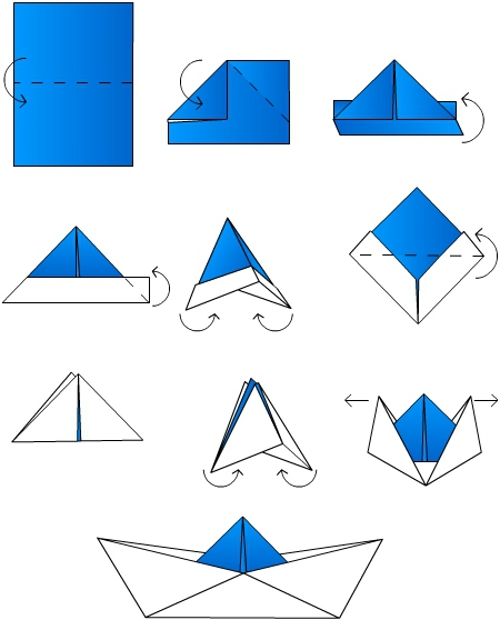
\includegraphics[angle=270, scale=0.03]{../Imagens/1.jpg} 

\label{figfrontal}
}
\subfloat[Vista esquerda]{

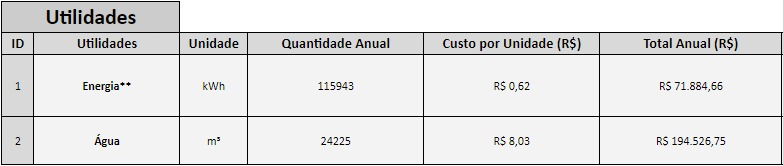
\includegraphics[angle=270, scale=0.03]{../Imagens/2.jpg} 

\label{figesquerda}
}

\subfloat[Vista direita/traseira]{

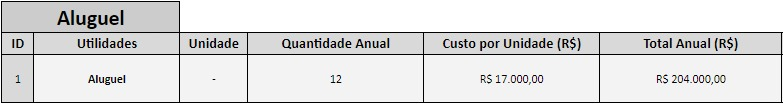
\includegraphics[angle=270, scale=0.03]{../Imagens/3.jpg}

\label{figdireita}
}

\subfloat[Vista superior]{

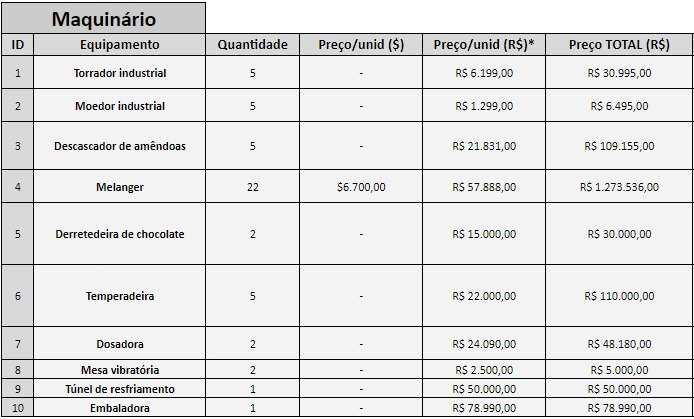
\includegraphics[angle=270, scale=0.03]{../Imagens/5.jpg}

\label{figsuperior}
}}

\caption{Vistas do robô montado}

\label{Img1}

\end{figure}

% ----------------------------------------------------------
% Capitulo com exemplos de comandos inseridos de arquivo externo 
% ----------------------------------------------------------

% ----------------------------------------------------------
% Parte de revisãod e literatura
% ----------------------------------------------------------


\newpage
\section[Resultados e Discussão]{Resultados e Discussão}
\pagestyle{fancy}

A partir dos tempos coletados durante a análise (Tabela \ref{t1}), calculamos as médias (Tabela \ref{t2}), por meio de média aritmética. (Abreviação de funcionário: func.)

\begin{table}[H]
\centering
\caption{Tempos coletados em segundos}
\vspace{0.5cm}
\begin{tabular}{c|c|c}

\textbf{1 func.} & \textbf{3 func. em fila} & \textbf{3 func. simultâneas}\\
\hline

19,34 & 13,49 & 11,22 \\ \hline
12,93 & 12,96 & 6,23 \\ \hline
14,62 & 10,73 & 5,29\\ \hline
11,61 & 23,31 & 5,12\\ \hline
11,22 & 10,36 & 5,20\\ \hline
12,62 & 9,50 & 4,35\\ \hline
35,55* & 21,79 & 4,65\\ \hline
12,44 & 13,22 & 4,46\\ \hline
11,78 & 24,76 & 4,91\\ \hline
14,74 & 11,70 & 5,50

\end{tabular}
\label{t1}
\end{table}

*Outlier

\begin{table}[H]
\centering
\caption{Médias calculadas em segundos}
\vspace{0.5cm}
\begin{tabular}{c|c|c}

\textbf{1 func.} & \textbf{3 func. em fila} & \textbf{3 func. simultâneas}\\
\hline

13,48 & 15,18 & 5,69 

\end{tabular}
\label{t2}
\end{table}

E a partir dessas médias de tempo($\overline{T}$) calculamos a produtividade mensal(P) de 1, 2 e 3 funcionários trabalhando em linha e simultaneamente. Para isso, consideramos um rendimento de 80$\%$, um dia contendo 25.200 segundos disponíveis e um mês apresentando 22 dias úteis.

\begin{center}

$P = \frac{25.200}{\overline{T}} \times 0,80 \times 22 \quad (1)$

\end{center}


A produtividade mensal (Tabela \ref{t3}) dos 4 casos foram alocados em uma tabela para melhor visualização.

\begin{table}[H]
\centering
\caption{Produtividade mensal em número de peças prontas}
\vspace{0.5cm}
\begin{tabular}{c|c|c|c}

\textbf{1 func.} & \textbf{2 func.} & \textbf{3 func. em fila} & \textbf{3 func. simultâneas} \\
\hline

32.902 & 65.804 & 29.217 & 77.947

\end{tabular}
\label{t3}
\end{table}

Considerando uma meta de 70.000 peças por mês e um salário de R$\$$1.000,00 mensal, com hora extra custando 50$\%$ a mais do que uma hora de trabalho normal, o custo total dos funcionários e suas horas extras são:

\begin{table}[H]
\centering
\caption{Custo total - META 70.000}
\vspace{0.5cm}
\begin{tabular}{c|c|c|c|c}

			 & \textbf{1 func.} & \textbf{2 func.} & \textbf{3 func. em fila} & \textbf{3 func. simultâneas} \\ \hline
\textbf{Produtividade} & 32.902 & 65.804 & 29.217 & 77.947 \\ \hline
\textbf{Peças faltando} & 37.098 & 4.196 & 40.783 & 0 \\ \hline
\textbf{Total dos Salários} & R$\$$1.000,00 & R$\$$2.000,00 & R$\$$3.000,00 & R$\$$3.000,00 \\ \hline
\textbf{Total das Horas Extras} & R$\$$1.302,29 & R$\$$147,29 & R$\$$1.612,19 & R$\$$0,00 \\ \hline
\textbf{Custo Total} & R$\$$2.302,29 & R$\$$2.147,29 & R$\$$4.612,19 & R$\$$3.000,00 

\end{tabular}
\label{t3}
\end{table}

Considerando uma meta de 170.000 peças por mês e um salário de R$\$$1.000,00 mensal, com hora extra custando 50$\%$ a mais do que uma hora de trabalho normal, o custo total dos funcionários e suas horas extras são:

\begin{table}[H]
\centering
\caption{Custo total - META 170.000}
\vspace{0.5cm}
\begin{tabular}{c|c|c|c|c}

			 & \textbf{1 func.} & \textbf{2 func.} & \textbf{3 func. em fila} & \textbf{3 func. simultâneas} \\ \hline
\textbf{Produtividade} & 32.902 & 65.804 & 29.217 & 77.947 \\ \hline
\textbf{Peças faltando} & 137.098 & 104.196 & 140.783 & 92.053 \\ \hline
\textbf{Total dos Salários} & R$\$$1.000,00 & R$\$$2.000,00 & R$\$$3.000,00 & R$\$$3.000,00 \\ \hline
\textbf{Total das Horas Extras} & R$\$$4.812,71 & R$\$$3.657,71 & R$\$$5.565,31 & R$\$$1.364,01 \\ \hline
\textbf{Custo Total} & R$\$$5.812,71 & R$\$$5.657,71 & R$\$$8.565,31 & R$\$$4.364,01 

\end{tabular}
\label{t4}
\end{table}

Com isso, podemos observar que a cronoanálise dentro de uma empresa faz total diferença no corte de custos e que devemos nos atentar para as características de cada empresa, pois cada análise foca diretamente naquilo que a empresa precisa, nos retornando resultados específicos. No caso da meta de 70.000 peças, verificamos que o melhor plano de produção ocorre quando possuímos 2 funcionários trabalhando em 2 peças distintas. Porém, no caso da meta de 170.000 peças, o melhor modelo para produção se encontra quando possuímos 3 funcionários trabalhando simultaneamente na mesma peça, dividindo o produto em setores que podem ser montados separados e depois ao final podem ser encaixados.

Em nossa simples análise não nos atentamos ao custo de estoque que poderia ocorrer caso algum modelo superasse a meta de produção, e nem ao máximo de horas extras que cada funcionário poderia realizar. Com isso, nossos resultados possuem um erro significativo se acaso os números de hora extra extrapolaram o limite determinado por lei, no entanto, podemos utilizá-los para comparação e análise dentro de um contexto que não contenha tais variáveis.


\newpage
% ---
\section[Conclusão]{Conclusão}
\pagestyle{fancy}% ---

Concluindo... bla bla

\postextual

% ----------------------------------------------------------
% Referências bibliográficas
% ----------------------------------------------------------
%\newpage
%\section[Referências Bibliográficas]{Referências Bibliográficas}
%\pagestyle{fancy}


% ----------------------------------------------------------
% Glossário
% ----------------------------------------------------------
%
% Consulte o manual da classe abntex2 para orientações sobre o glossário.
%
%\glossary

\end{document}
